\documentclass[tikz]{standalone}
\usetikzlibrary{positioning,arrows}
\begin{document}
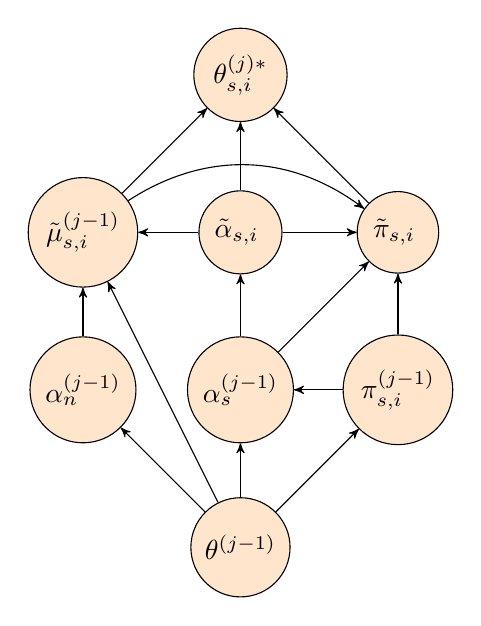
\begin{tikzpicture}
% Draw Graphical Model
   \begin{scope}[ node distance=2cm,on grid,>=stealth',
                   block/.style={rectangle,draw,fill=cyan!20},
                   comp/.style={circle,draw,fill=orange!20} ]
     \node [comp]  (main)                    {$\theta_{s,i}^{(j)*}$};
     \node [comp]  (c1)   [below=of main]   {$\tilde\alpha_{s,i}\;$} edge [->] (main);
     \node [comp]  (c2)   [right=of c1]       {$\tilde\pi_{s,i}\;$} edge [->] (main);
     \node [comp]  (c3)   [left=of c1]   {$\tilde\mu_{s,i}^{(j-1)}$} edge [->] (main);
     \draw (c1) edge [->] (c2);
     \draw (c1) edge [->] (c3);
     \draw (c3) edge [->,bend left=35] (c2);
     \node [comp]  (c5)   [below=of c3] {$\alpha_{n}^{(j-1)}$} edge [->] (c3);
     \node [comp]  (c6)   [below=of c1] {$\alpha_{s}^{(j-1)}$} edge [->] (c2);
     \draw (c6) edge [->] (c1);
     \node [comp]  (c7)   [below=of c6] {$\theta^{(j-1)}$} edge [->] (c3);
     \draw (c7) edge [->] (c5);
     \draw (c7) edge [->] (c6);
     \node [comp]  (c8)   [right=of c6] {$\pi_{s,i}^{(j-1)}$} edge [->] (c6);
     \draw (c7) edge [->] (c8);
     \draw (c8) edge [->] (c2);
     % \node [comp]  (c9)   [below=of null]   {!} edge [->] (null);
     % \node [comp]  (c10)  [below=of null]   {!} edge [->] (null);
     % \node [comp]  (c11)  [below=of null]   {!} edge [->] (null);
     % \node [comp]  (c12)  [below=of null]   {!} edge [->] (null);
     % \node [comp]  (c13)  [below=of null]   {!} edge [->] (null);
     % \node [block] (p1)   [below=of c1]       {$\alpha$} edge [->] (c1);
     % \node [block] (p2)   [below=of c2,xshift=-0.8cm]       {$\beta$} edge [->] (c2);
     % \node [block] (p3)   [right=of p2]       {$\gamma$} edge [->] (c2);
     % \node [comp]  (c7)   [below=of null]   {!} edge [->] (null);
   \end{scope}
\end{tikzpicture}
\end{document}

%%% Local Variables: 
%%% mode: latex
%%% TeX-master: t
%%% End: 
